\pagestyle{fancy}
\rhead{\thepage}
\lhead{Study 2: User Study}
\chapter{Study 2: User Study}
\label{ch: chapter 4}

Following the first study (See Chapter \ref{ch: chapter 3}), A laboratory study was conducted to evaluate user experience on different design patterns of music sequencers. In section \ref{subsec: representative}, one representative sequencer application was chose from each interface category presented in the first study. Based on the previous work of evaluating music NIME, a questionnaire was designed to measure muscians experience (See Section \ref{subsec: questionnaire}).

\section{Method}
\subsection{Representative Sequencer Applications}
\label{subsec: representative}

Considering the duration of the user study, we decided to select three apps that can represent it\textquotesingle s own group most. In order to pick one representative application from each group, we first selected several apps from each category. Then, in order to eliminate the unnecessary disruptive factors such as the robustness of apps, the application shared the similar building quality were chose. In the end, \textit{S.A.M.M.I} from the traditional category, \textit{Beatwave} from the multi-track and \textit{Volotic} from the novel category were chose to use in the user study.

In addition, took the influence of the presenting order of the above three apps in consideration, we futher disrupt the order of these three sequencer apps in the user stury.

\subsection{Questionnaire}
\label{subsec: questionnaire}
Likert scale questionnaire is widely used approach to represent people's reponse to a topic. For each topic there are normally five satisfaction items used to describe people's feeling. And a satisfaction item is a number between one to five, which represents interviewee's level of agreement over the topic. The higher number a topic scored means the more the interviewee agreed with it. Based on \citeauthor{Reference0}'s work, which developed a 80-item pool ordered by descending mean importance for questionnaire, 10 questions that scored the highest mark from 9 different categories were used in the user study (see Appendix \ref{app:Appendix A}).

\begin{table}[h]

  \begin{tabular}{ |p{1.2cm}|p{2.5cm}|p{9.2cm}|p{0.6cm}|}
   \multicolumn{4}{l}{} \\
   \hline
   Factor & Category  & Item  & $\mu$ \\
   \hline
   EFP & Creativity & The instrument allows me to be creative & 6.25\\
   & Enjoyment &  I have fun playing the instrument & 6.08\\
   & Expressiveness & The instrument allows me to express myself & 6.06\\
   \hline
   PCC & Conformance & The instrument responds well to my actions & 6.23\\
   & Control & I can control the sound appropriately & 6.04\\
   & Engagement & The instrument allows me to be engaged when I'm playing it & 5.98\\
   & Engagement & I feel the urge to play the instrument again & 5.79\\
   & Play Comfort & I can recognize that the instrument responds well to my playing & 5.85\\
   \hline
   PSSQA & Stability & I can rely on the instrument when playing it & 6.21\\
   & Sound Quality & The instrument pleases me sound-wise & 6.02\\
   \hline
  \end{tabular}
  \caption[l]{Items in the questionnaire with thier factor and category(ordered by descending mean importance)}
  \label{tab: questionnaire}
\end{table}

Follow the framework of MPQ-Q questionnaire, 10 questions from 3 factors were implemented in our questionnaire(see Table \ref{tab: questionnaire}). For each factor, only the items score the highest mean importance value in the certain category were picked. Under the EFP factor, we focused at the creativity, enjoyment and expressiveness of the music sequencer. The reason for this, it's because we want to figure out whether the design of the interface is encouraging musicians to explore new possibilities and inspiring musicians' creativity. As for the PCC, items associate with conformance, control and engagement are chose. The reason behind this is when musicians performing on instruments there are a lot of physical interaction between musicians and instruments, whether the musiciain feel conformance and engagement have impact on their overall satisfaction. For items under PSSQA, we only look at the stability and sound quality. Because the more stable of the music sequencer the more confident musicians can rely on it. Same with the sound quality, only the instrument that can satisfy the muscian is able to please the audience.

\subsection{Participants}

In total, twenty participants with different music background were invited and took part in the user study. Fifteen of them are male and five are female. All the participants have at least one year of formal training on at least one instrument. Among the participants, the majority only had experience with traditional instruments such as piano, guitar and violin. Only three musicians had experience on electronic music and had tried on music sequencer software on the laptop before. All musicians still play music regularly.

\bigskip
\begin{figure}[h]
  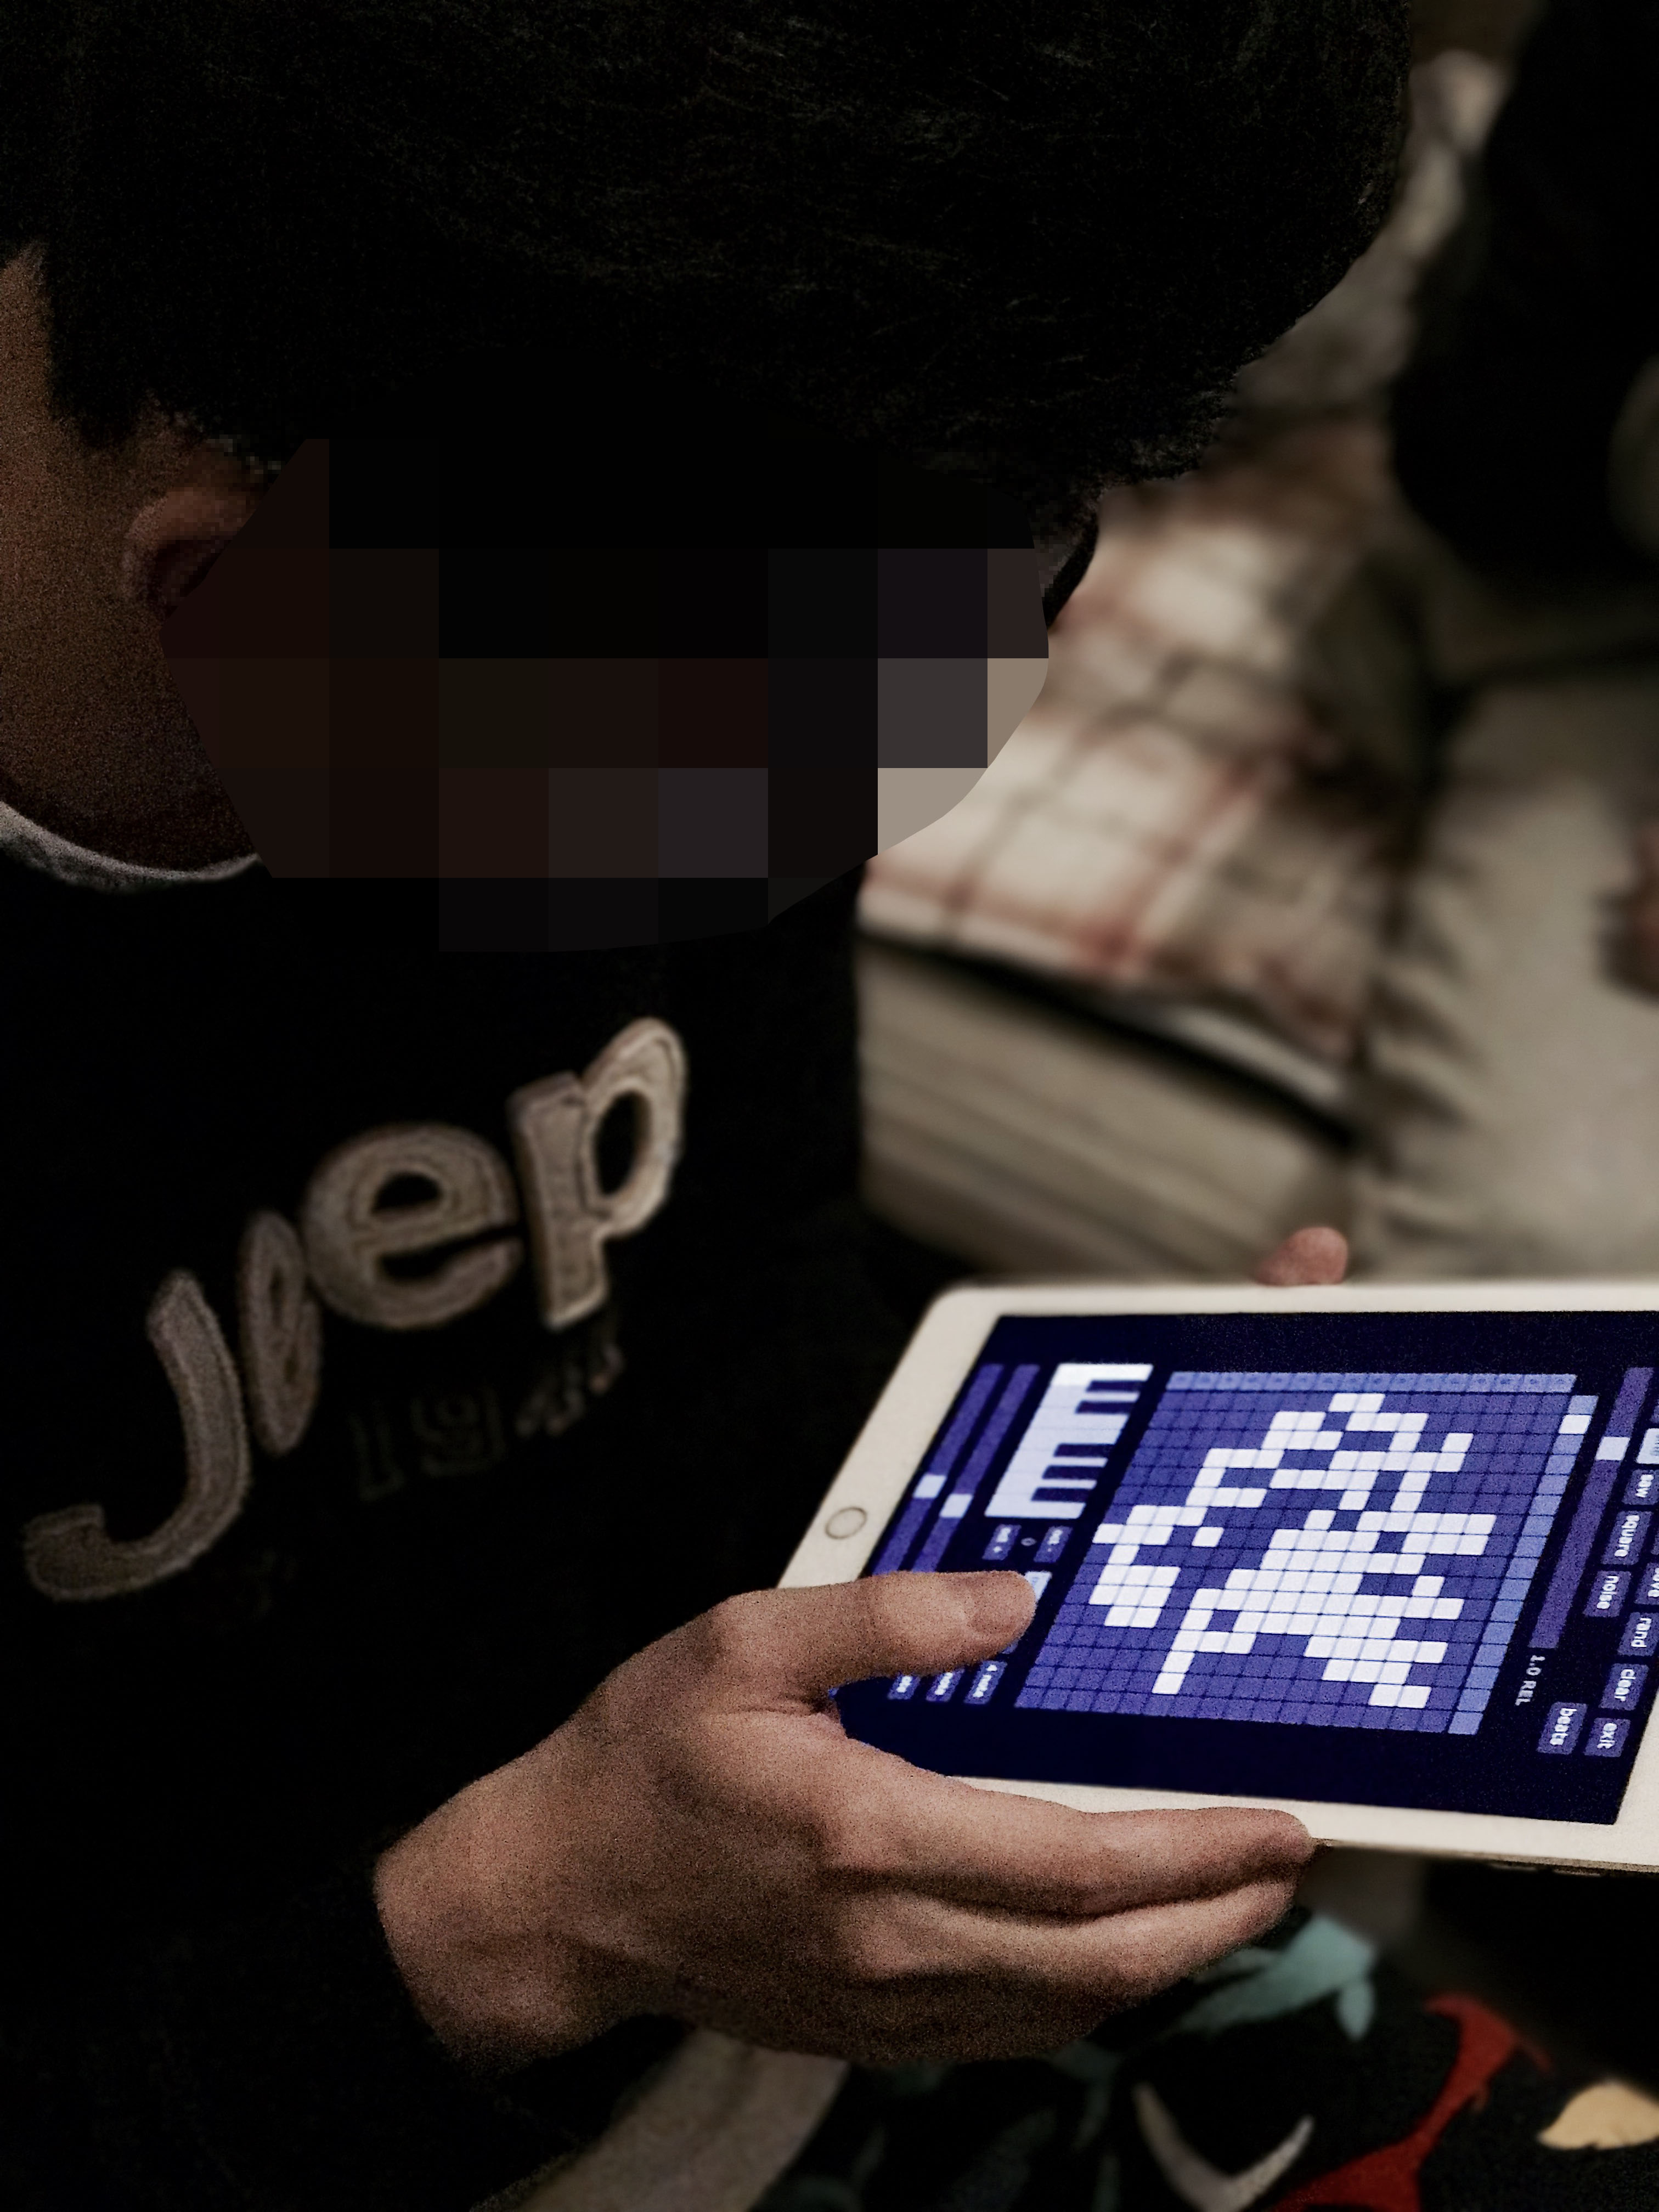
\includegraphics[width=6cm]{images/Participant}
  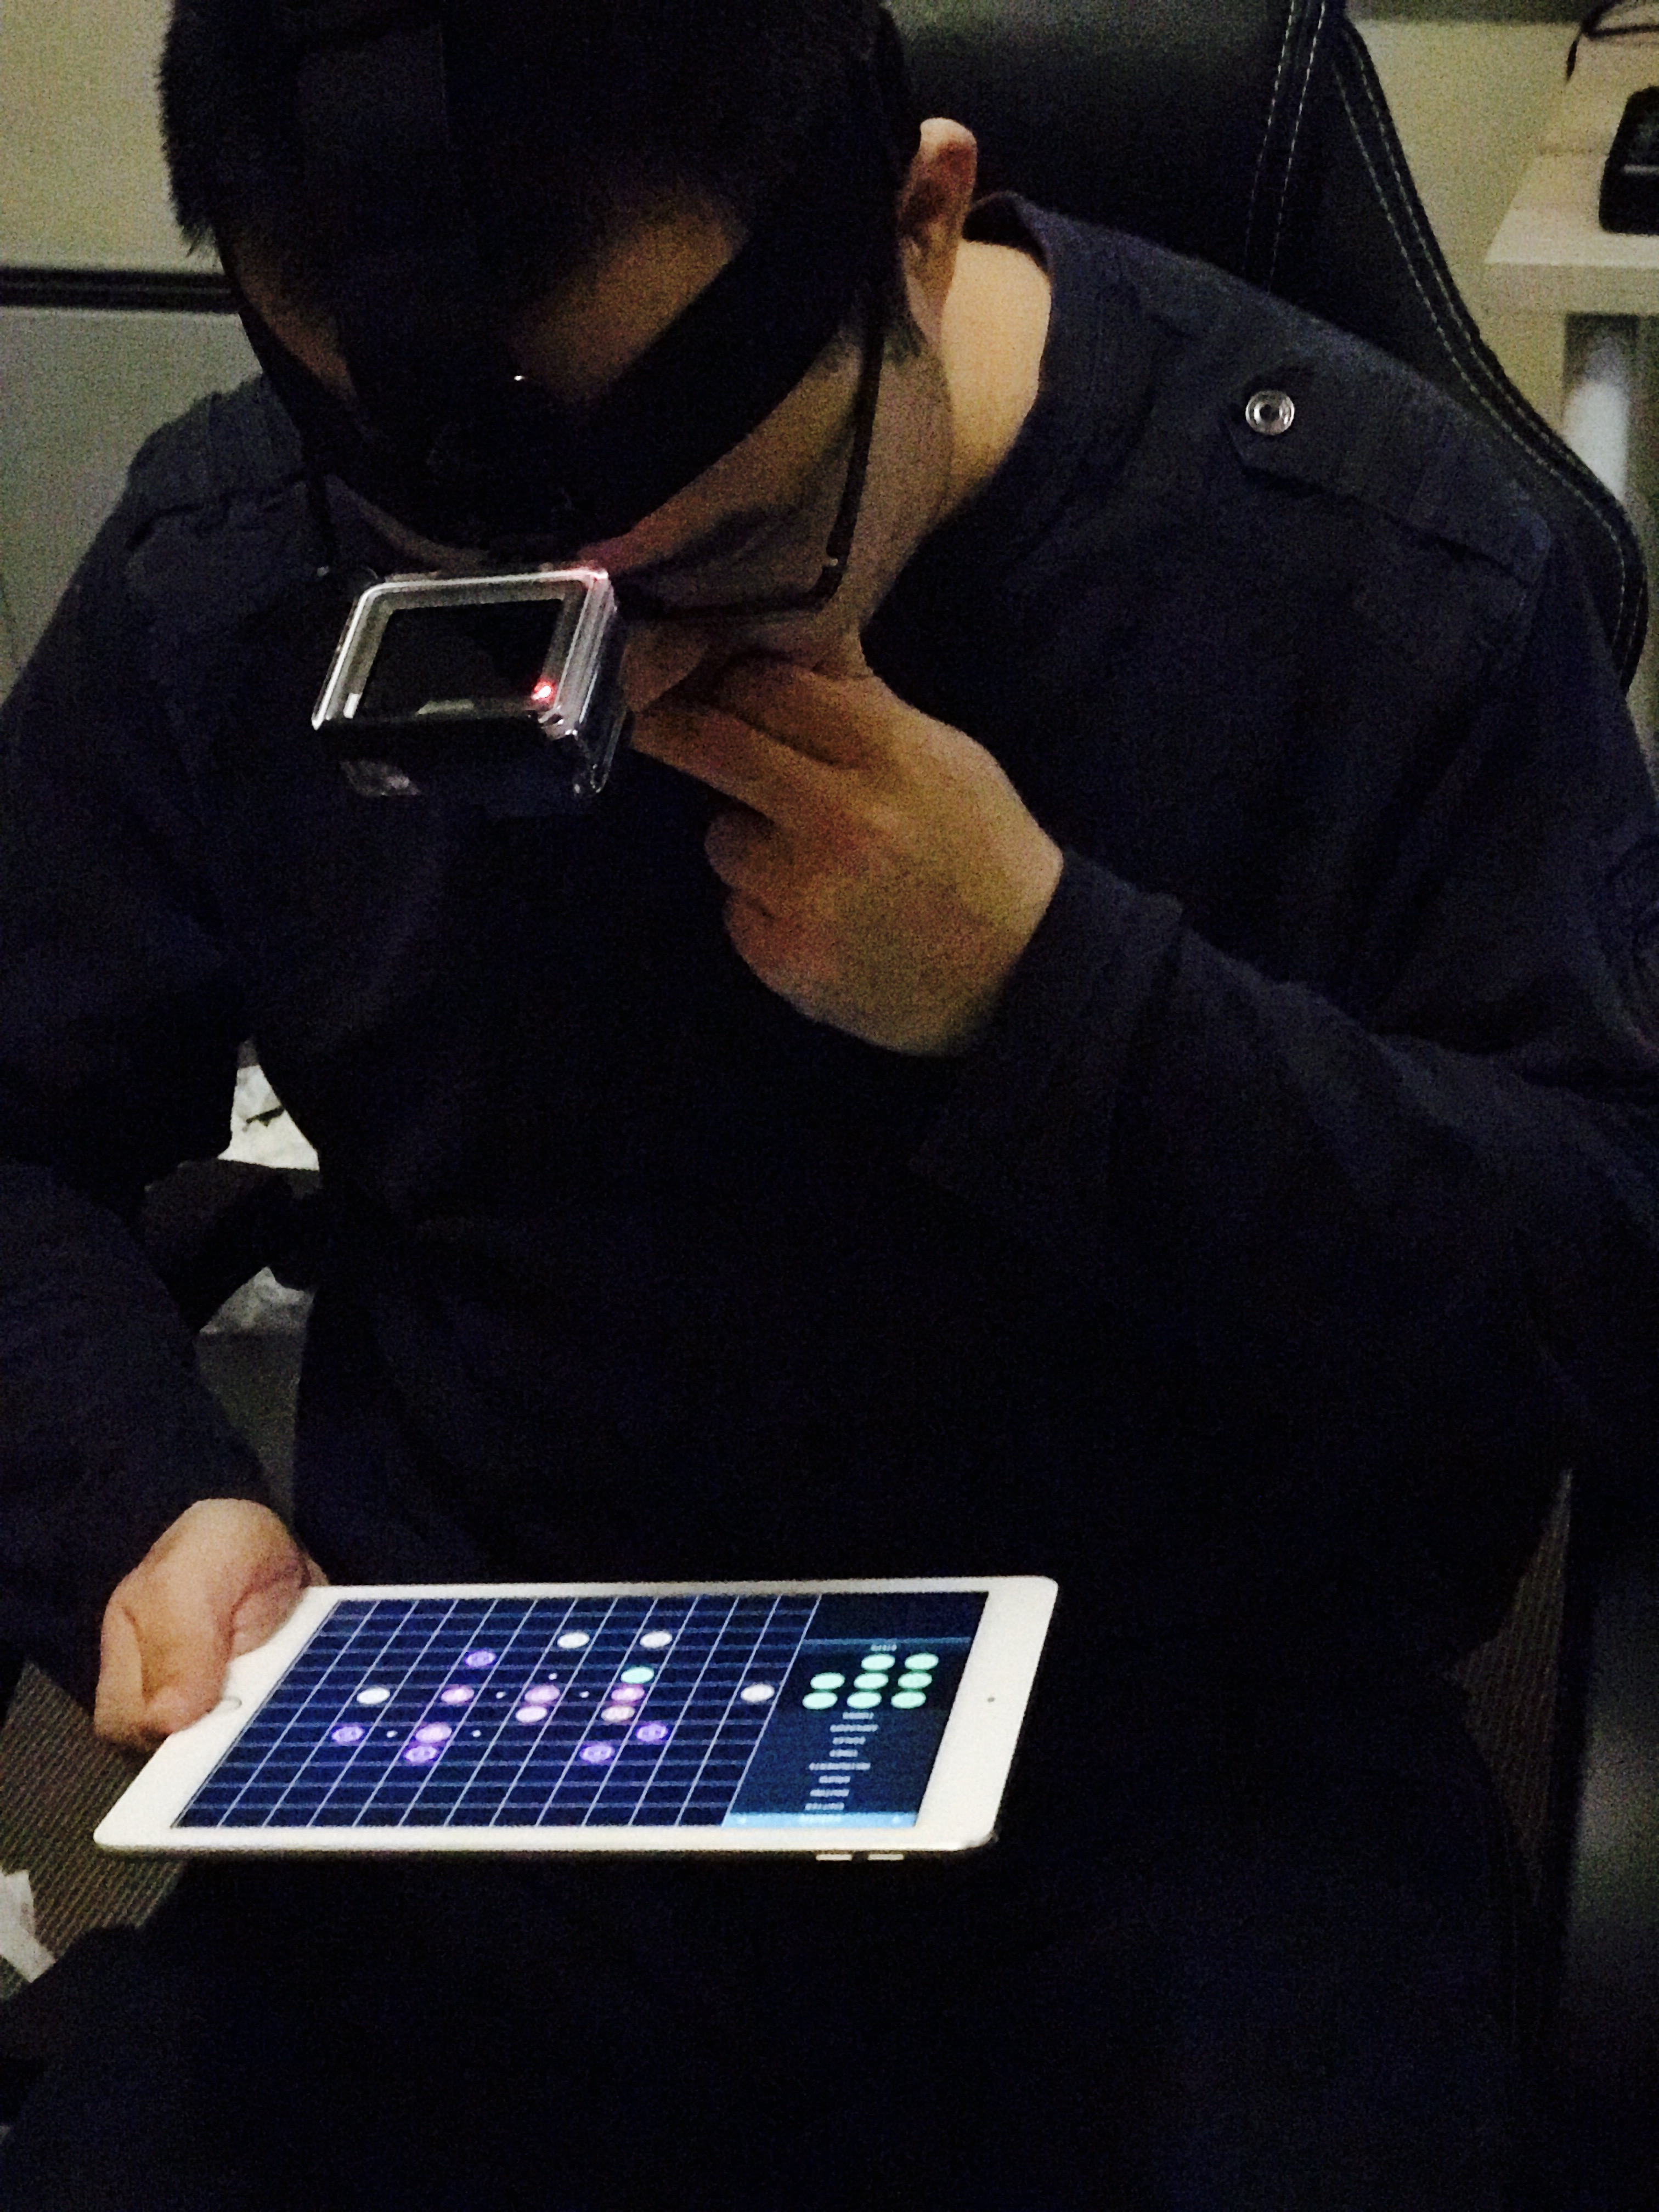
\includegraphics[width=6cm]{images/Participant2}
  \centering
  \caption{Participants test on the music sequencer on iPad}
  \label{fig: participant}
\end{figure}
\bigskip

\section{User Study Process}

The duration of the user study was planned as approximately one hour. The first fourty-five minutes was the try-on section which quantitively analyzed the interface (see \ref{subsec: play on}). In the last fifteen minutes, an interview was designed for qualitative analysis purpose (see \ref{subsec: interview}).

\subsection{Apps try-on}
\label{subsec: play on}
In this try-on section, all the participants were asked to play on the selected music sequencer applications on iPad. For each apps, musicians were given 15 minutes to explore the apps by themselves, and assistance was given only in request. The suggested time allocation was given as: in the first five minutes try to figure out the how it works, then impovise with the apps in the next ten minutes. After trying on each sequencer application, participants will be given a questionnaire with 10 questions to decide their feelings on the app in terms of expressivity, control and aesthetic(see Appendix \ref{app: Appendix B}).


\subsection{Interview}
\label{subsec: interview}
Participants were intervied at the end of the user study. The main purpose of the interview is to find out the reason behind their decision on the questionnaire. Besides, the music background of participants such as \textit{\textquotedblleft{how many years of music training}\textquotedblright} were recorded for further analysis. The sample question was given in the appendix \ref{app: AppendixC}.

In order to acquire the deeper reason, all the interview followed the same procedure: 1) Since the majority of the participants did not know music sequencer before, they were asked to describe the similarities among the three different music sequencer applications, and then defined what is music sequencer. which was designed to help them to form a general idea of music sequencer. 2) After that, interviewees were asked to choose their favourite application based on different scenario. Also, the interviewee needed to give reasons why certain music sequencer application was better than another. 3) In the final step, all the questions shifted to an abstract level, where they were asked whether music sequencer application on iPad were an instrument ,and what features that made them thought it is or it is not an instrument.The interviews were recorded on video and audio based on the participants agreement. The recording lasted between 10 to 20 minutes.

\section{Results}

\emph{My supervisor (Dr. Ben Swift) assisted in the preparation of the graphs
and statistical tests discussed in this section.}

\subsection{Quantitative Results}

In total, 600 satisfaction items from twenty participants were extracted from the questionnaires (The raw data was attached in Appendix \ref{app: Appendix D}). A statistic analyze of the data was divided into three group, which based on the factor of questions. Figure \ref{fig: result_EFP} shows the questions under EFP and specific distribution of agreement level over the selected apps. Similar to figure \ref{fig: result_PCC} which shows results over question related to PCC, and figure \ref{fig: result_PSSQA} is the collection of results associated with PSSQA.


\bigskip
\begin{figure}[h]
 \centering
 \includegraphics[width = \textwidth]{figs/responses-by-question-Q01.pdf}
 \includegraphics[width = \textwidth]{figs/responses-by-question-Q04.pdf}
 \includegraphics[width = \textwidth]{figs/responses-by-question-Q05.pdf}
 \caption{Participants response on questions under EFP}
 \label{fig: result_EFP}
\end{figure}
\bigskip
\begin{figure}
 \centering
 \includegraphics[width = \textwidth]{figs/responses-by-question-Q02.pdf}
 \includegraphics[width = \textwidth]{figs/responses-by-question-Q06.pdf}
 \includegraphics[width = \textwidth]{figs/responses-by-question-Q08.pdf}
 \includegraphics[width = \textwidth]{figs/responses-by-question-Q09.pdf}
 \includegraphics[width = \textwidth]{figs/responses-by-question-Q10.pdf}
 \caption{Participants response on questions under PCC}
 \label{fig: result_PCC}
\end{figure}

\begin{figure}[h]
 \centering
 \includegraphics[width = \textwidth]{figs/responses-by-question-Q03.pdf}
 \includegraphics[width = \textwidth]{figs/responses-by-question-Q07.pdf}
 \caption{Participants response on questions under PSSQA}
 \label{fig: result_PSSQA}
\end{figure}

\subsection{Qualitative Results}

The result in this section is based on the information extracted from the interview. A summary of results is presented in table \ref{tab: suduko}.

\textbf{S.A.M.M.I}\qquad Musicians find \textit{S.A.M.M.I} is very easy to use becasue of the intuitive design of interface. Although \textit{S.A.M.M.I} does not provide much options in terms of variety of sounds and adjustment over the sound effect, it is complex enough for most of participants to master this instrument in such a short time. Besides, thanks to the annotation of different pitch, \textit{S.A.M.M.I} is the only application that musicians were confident enough to create a short piece of melody, such as theme music of \textquotedblleft{Super Mario}\textquotedblright and \textquotedblleft{Mary Had a Little Lamb}\textquotedblright. Because of it's explicit layout of control panel and simultaneous reponse over the operation, one musician suggested to use \textit{S.A.M.M.I} in live music performance.

\textbf{Beatwave.}\qquad The comments on \textit{Beatwave} are mainly focused on the layout of different tracks. They agree on combining severl layers of music together is definitely an improvement, but this design pattern makes it more difficult to control comparing with the single-track interface of \textit{S.A.M.M.I}. Moreover, some musicians think the multi-track interface is very useful in composing music with different sounds mix together. The opinion on the visual effect of \textit{Beatwave} is divided. Most musicians support the rippling visual effect for it helps them track down the current process of music. But a few musicians disagree and think it does not have actual effect on composition.

\textbf{Volotic.}\qquad \textit{Volotic} is recognized as the most difficult application to create music. Mostly because timing in \textit{Volotic} is controled by the time a signal(or little dots) travels in the interface. However, it turns to be diffcult to control when there are several little dots travelling on the screen. Participants share the same reaction  over \textit{Volotic}, \textquotedblleft{It's more like a game rather than an instrument}\textquotedblright. But they still think it is a very good practice and could potentially used to help kids generate interest in music.

\begin{table}[h]
  \centering
  \begin{tabular}{ |p{2cm}|p{3.2cm}|p{3.2cm}|p{3.2cm}|}
   \multicolumn{4}{c}{} \\
   \hline
   \rowcolor{gray!50}
   Types &  Expressivity  &  Control  &  Aethetic \\[2ex]
   \hline
   & & & \\
   Traditioanl (S.A.M.M.I) & $\bullet$ can not fully express myself & $\bullet$ very easy to learn & $\bullet$ the interface is dull\\
   & $\bullet$ feel boring in a short time &  $\bullet$ the design is itutive & $\bullet$ appearence is not appealling\\
   & & &\\
   \hline
   & & &\\
   Multi-track  (Beatwave)& $\bullet$ it inspires my creativity & $\bullet$ not easy to get start & $\bullet$ the interface loos awesome\\
   & $\bullet$ a feel I can do more& $\bullet$ the layout is somehow confusing & $\bullet$ the visual effect is very helpful\\
   & & &\\
   \hline
   & & &\\
   Novel  (Volotic)& $\bullet$ kind of inspiring creativity & $\bullet$ very confusing & $\bullet$ it looks interesting\\
   & $\bullet$ it's fun & $\bullet$ would be better with an instruction & $\bullet$ the interface looks like a game\\
   & & &\\
   \hline
  \end{tabular}
  \caption{ Musicians opinions summarised from the interview}
  \label{tab: suduko}
\end{table}

\subsection{Discussion}

When dealing with statistical significance and Likert scale responses,it is important not to make assumptions of the data which are not true in the likert case\citep{norman_likert_2010}. The Aligned Rank
Transform\citep{wobbrock_aligned_2011} (ART) has become popular in the CHI community to perform non-parametric factorial analyses of likert responses. Although finding statistical significance is not the main
point of this user study, an ART was performed (using the R ARTool package\citep{matthew_kay_2016_48543}) to see if there was any difference in the responses between the apps. Table \ref{tab: p-value} shows the results after applying a Bonferroni correction to account for multiple tests. In the table the questions in shade were regarded as not significant, because the adjusted p-value of these two question were greater than 0.05.

\bigskip
\begin{table}[ht]
\rowcolors{2}{gray!25}{gray!25}
\begin{tabular}{p{12cm} p{1.5cm}}
 \hline
 \rowcolor{gray!50}
Questions & adjusted \textit{p-value} \\
\hline
\hiderowcolors The instrument allows me to be creative & 0.0014 \\
\hiderowcolors The instrument responds well to my actions & 0.0234 \\
\hiderowcolors I can rely on the instrument when playing it & 0.0009 \\
\showrowcolors I have fun playing the instrument & 0.3093 \\
\hiderowcolors The instrument allows me to express myself & 0.0010 \\
\hiderowcolors I can control the sound appropriately & 0.0009 \\
The instrument pleases me sound-wise & 0.0121 \\
\hiderowcolors I feel the urge to play the instrument again & 0.0486 \\
\showrowcolors The instrument allows me to be engaged when I'm playing it & 0.1523 \\
\hiderowcolors I can recognize that the instrument responds well to my playing & 0.0006 \\
\hiderowcolors
\hline
\end{tabular}
\caption{Questions with adjusted p-value.}
\label{tab: p-value}
\end{table}

From the statistic results extracted from the questionnaire, it is clear to say that the multi-track interface represented by \textit{Beatwave} is the most popular design among musicians. By contrast, the non-traditional interface represented by \textit{Volotic} received most of the nagative comments.

Considering the factor each question belong to (see Table \ref{tab: questionnaire}), we can look in details of what specific aspect an interface good at. In Figure \ref{fig: EFP}, statistic result for questions belong to \textit{EFP} were grouped together. Apparently, \textit{Beatwave} was the best applcation to encourage musicians creativity. And \textit{Volotic} was slightly better than \textit{S.A.M.M.I} in this category. In enjoyment category, \textit{Beatwave} still gathered most of \textquotedblleft{Strong Agreement}\textquotedblright. But \textit{Volotic} was not that fun compaied with \textit{S.A.M.M.I}. For the expressiveness of the applications, \textit{Beatwave} and \textit{S.A.M.M.I} were quite similar, the only difference was musicians had stronger feeling on \textit{Beatwave}. However, opinions on \textit{Volotic} were equally distributed, it looked like musicians had a substential differences on whether the interface of \textit{Volotic} supported them to expressed themselves.
%
% \bigskip
% \begin{figure}
% \begin{minipage}[b]{0.5\textwidth}
% 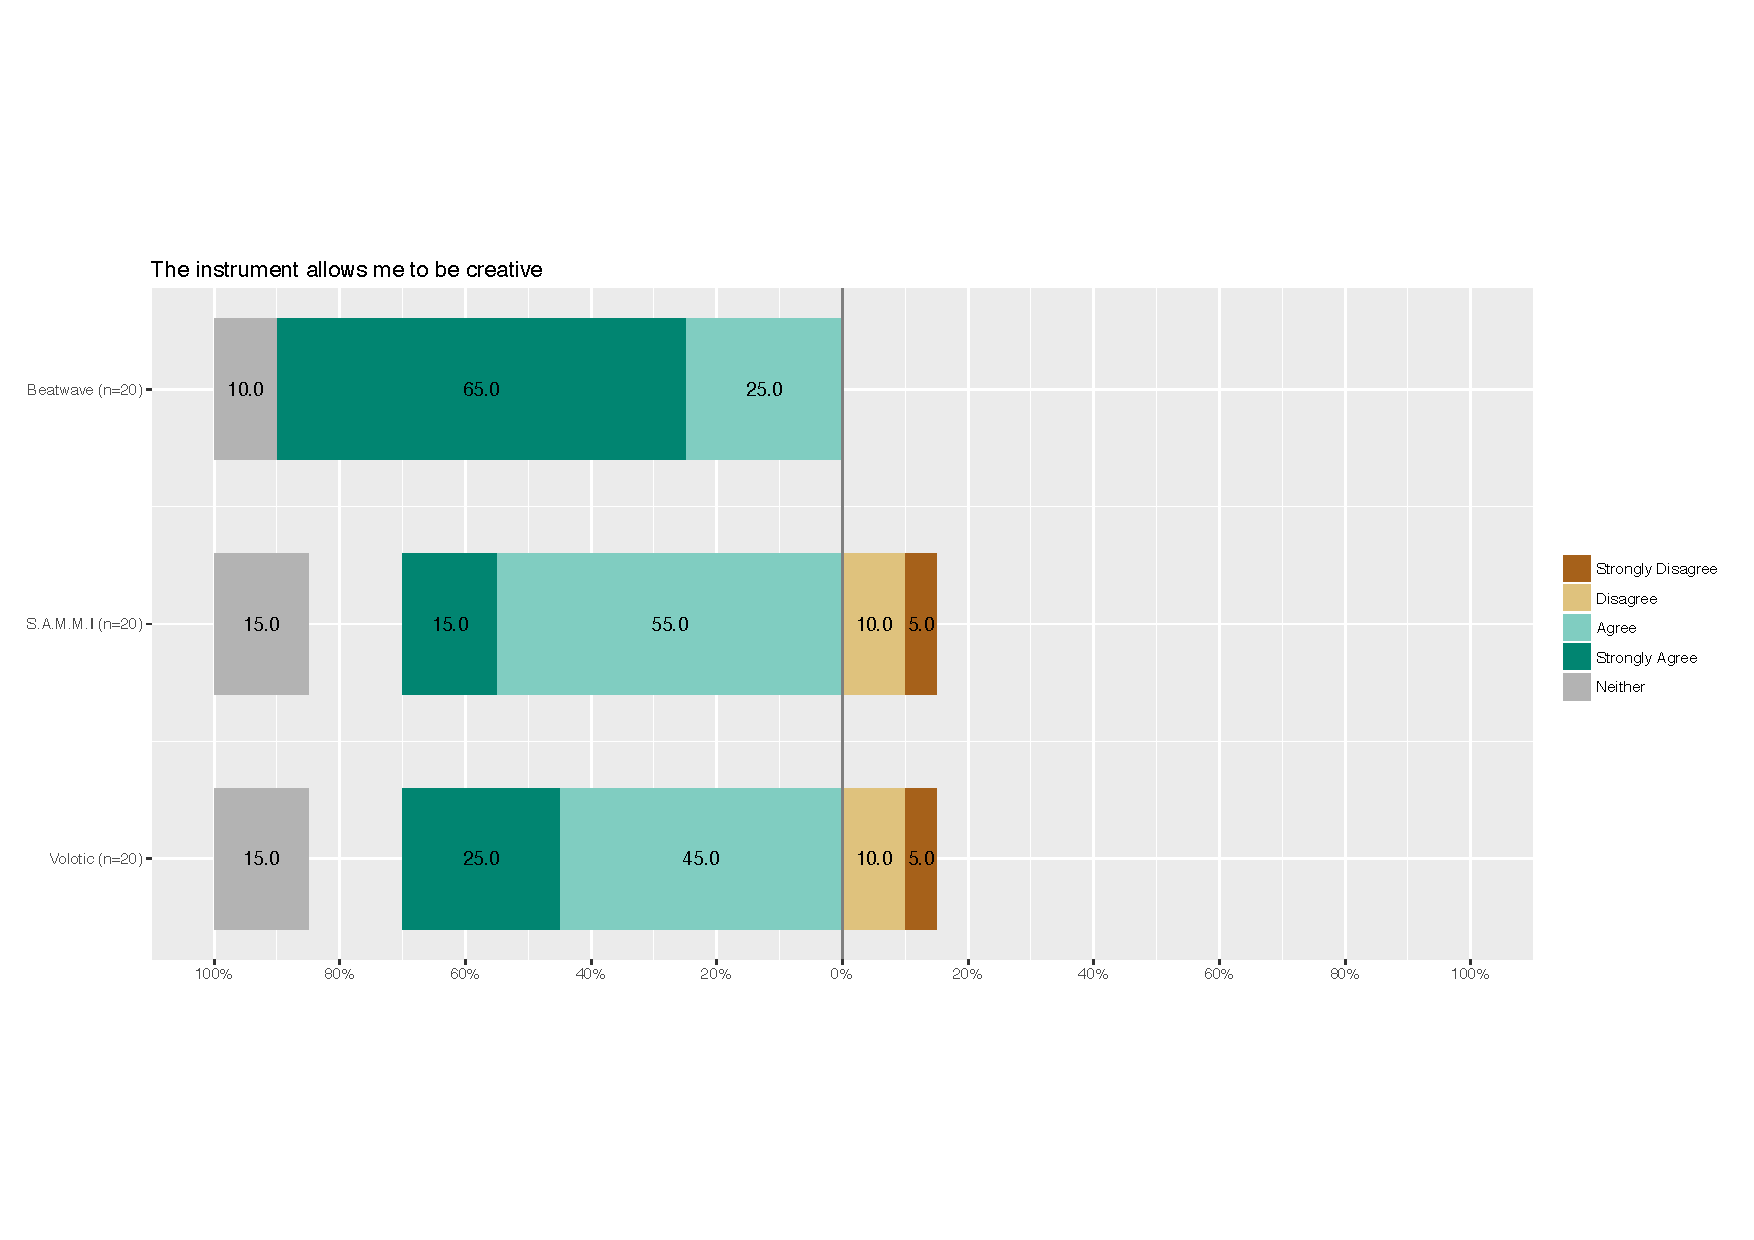
\includegraphics[width=\linewidth]{figs/Q1.pdf}
% \end{minipage}
% \begin{minipage}[b]{0.5\textwidth}
% 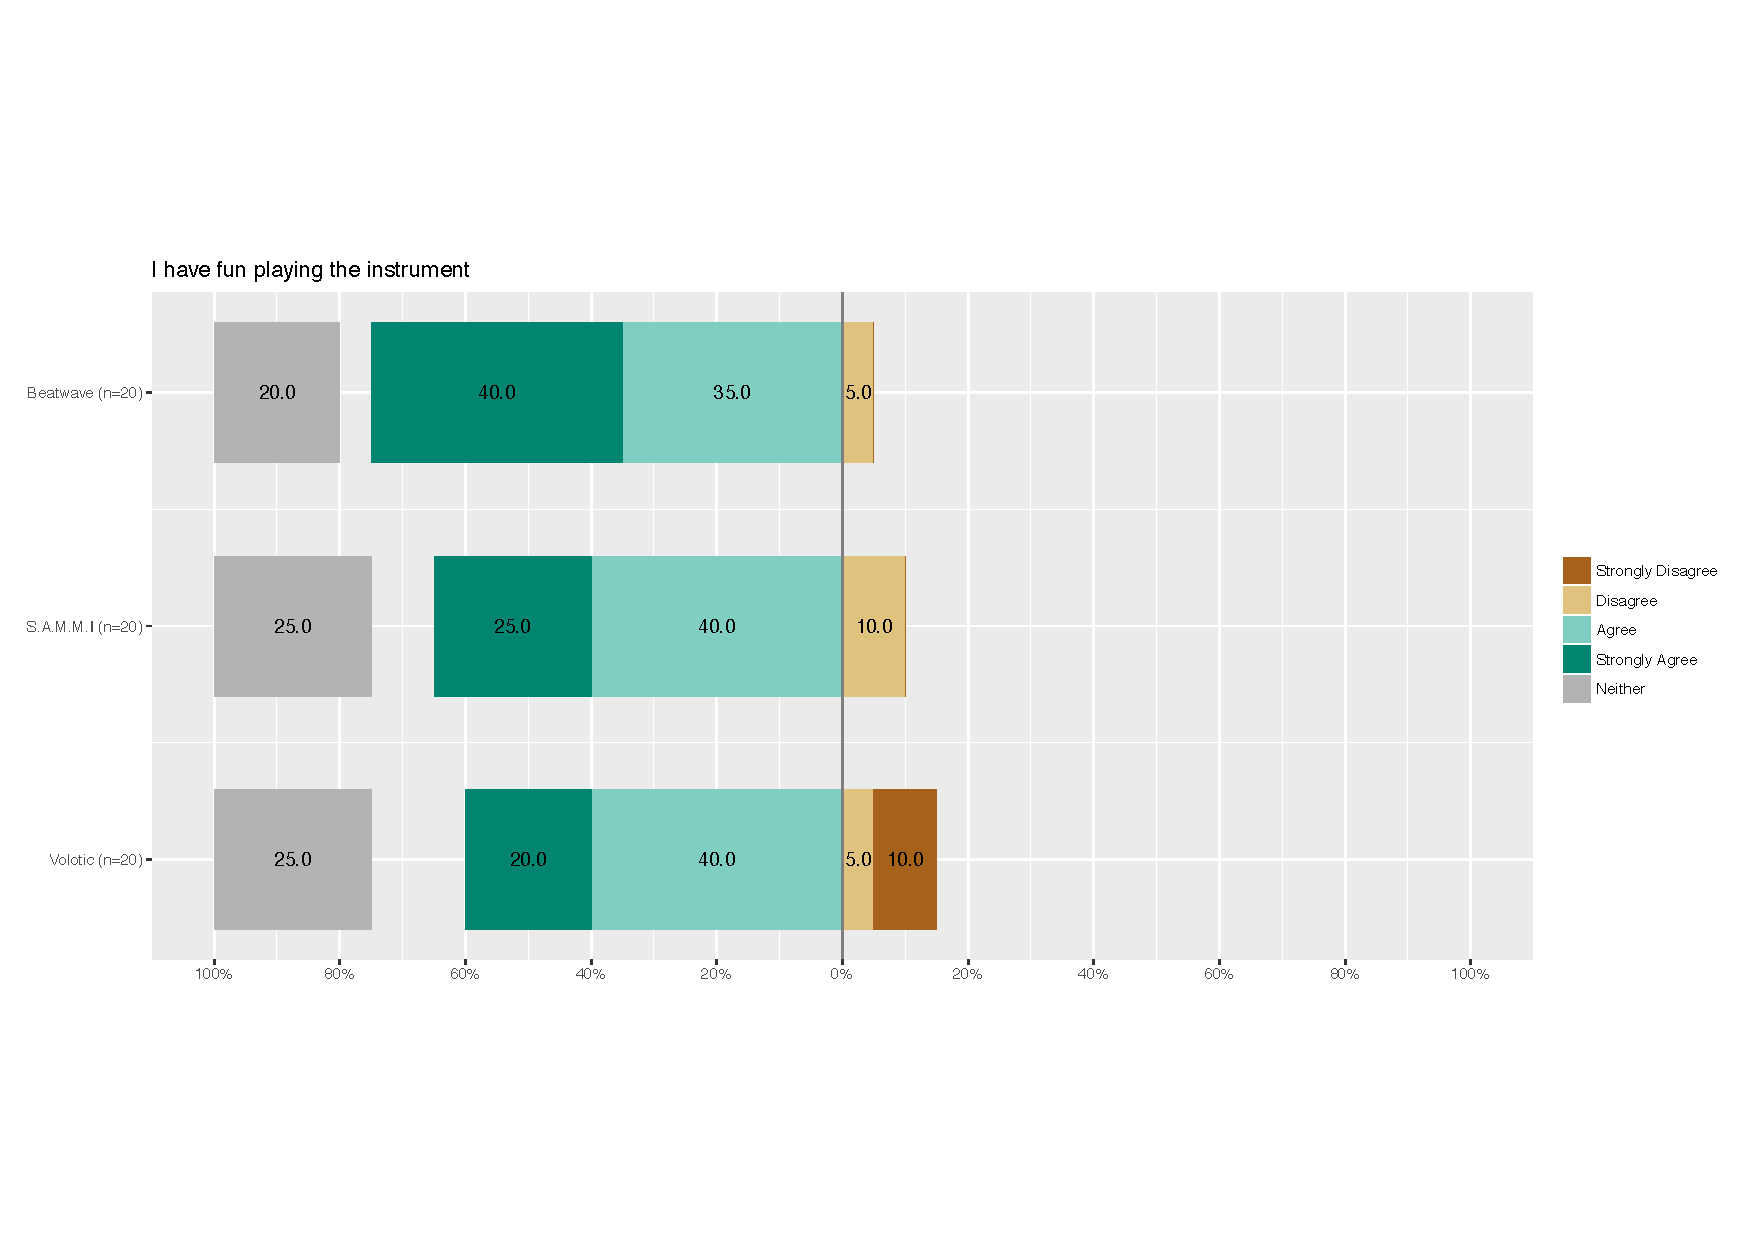
\includegraphics[width=\linewidth]{figs/Q4.pdf}
% \end{minipage}
%
% % \hspace{\fill}
%
% \begin{minipage}[b]{0.5\textwidth}
% 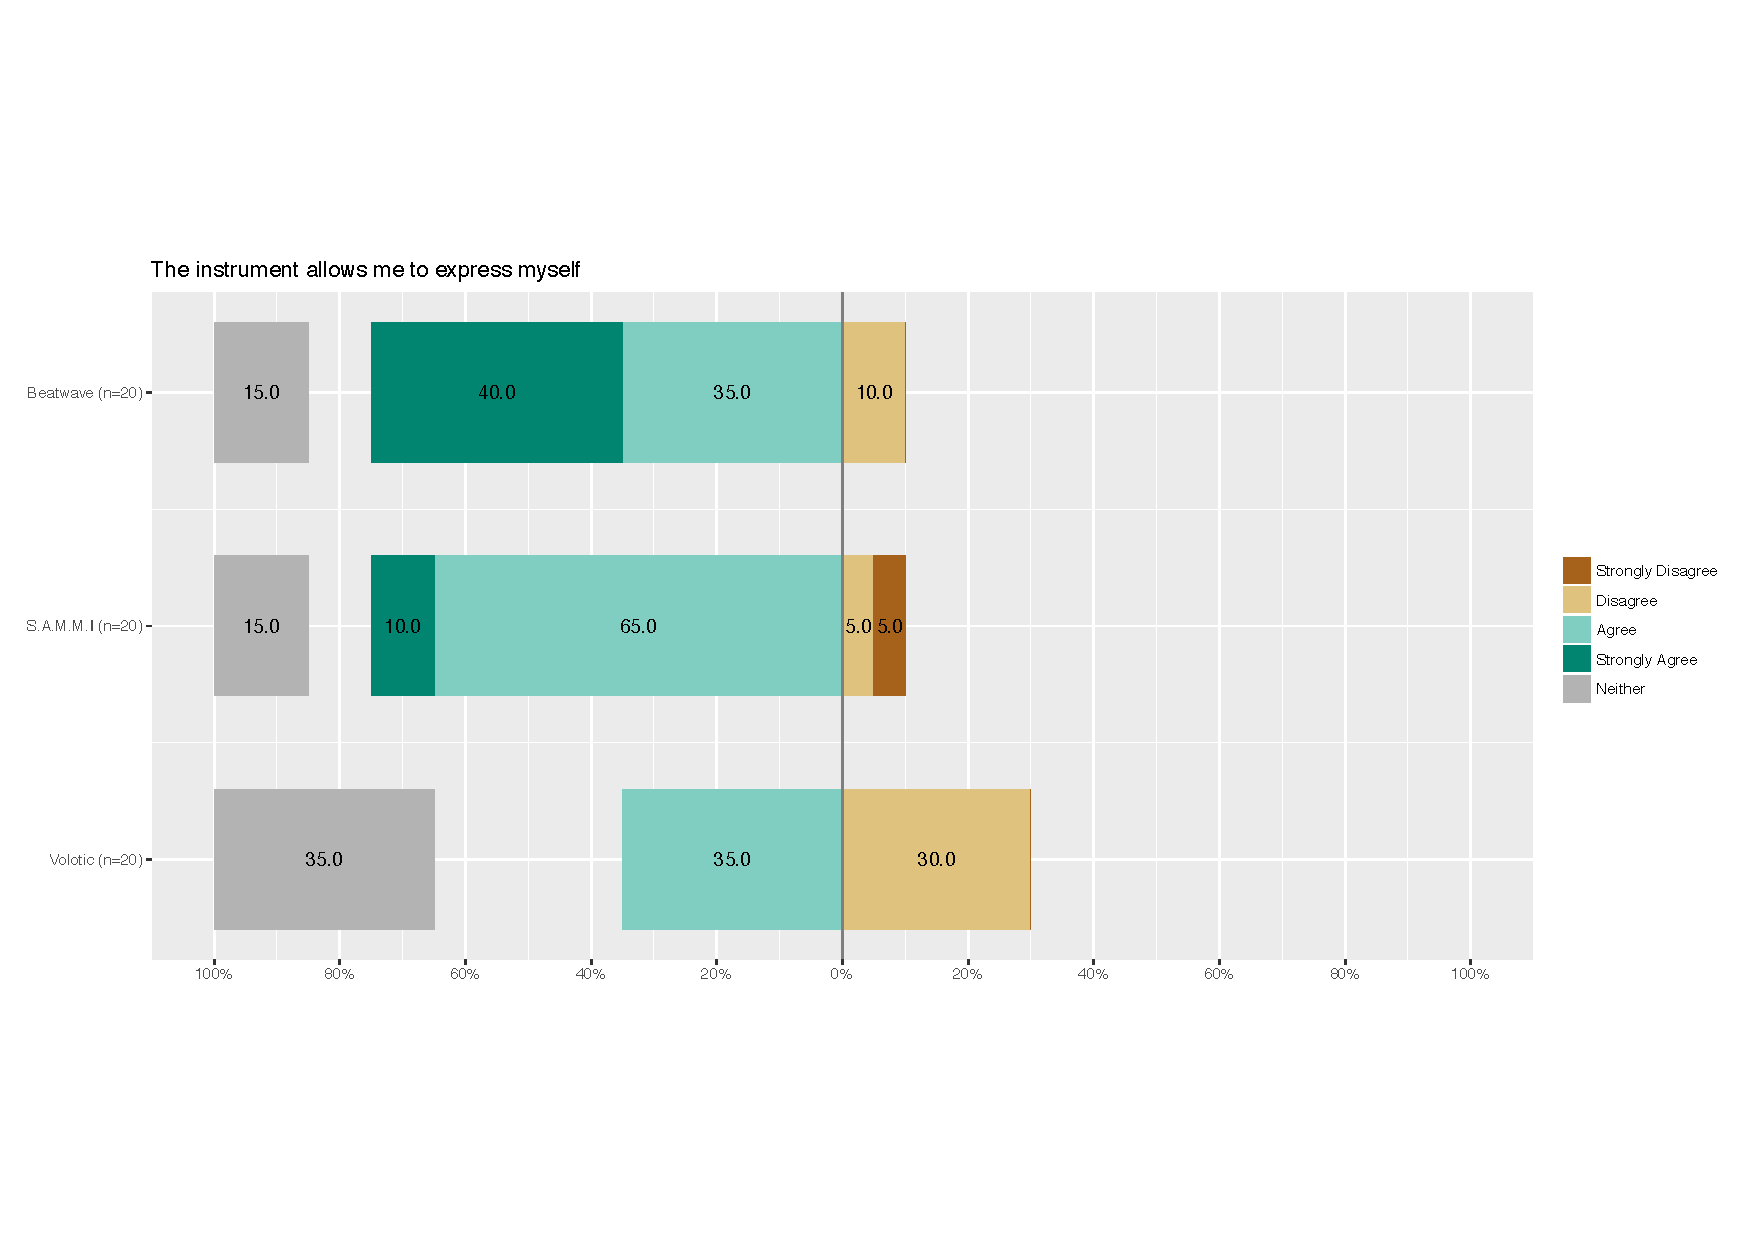
\includegraphics[width=\linewidth]{figs/Q5.pdf}
% \end{minipage}
% \begin{minipage}[b]{0.5\textwidth}
% 
\includegraphics[width=\linewidth]{figs/Q0.pdf}
% \end{minipage}
%
% \caption{Statistic results for questions belong to \textit{EFP}}
% \label{fig: EFP}
% \end{figure}
% \bigskip


\clearpage
